\newpage
\subsection{Satellite Number Variations}
This series of tests involved evaluating the effect of changing the number of satellites in the constellation on the performance metrics outlined in Section \ref{sec:perfMetrics}. The same three-plane orbital configuration was kept from Table \ref{tab:satRefCase}, whilst the number of satellites per-plane were changed. 
\subsubsection{Input Variables}
From the reference case specified in Table \ref{tab:satRefCase}, the number of satellites per each of the 3 planes were varied between 1 and 6 according to Table \ref{tab:perPlaneParams}.

\begin{table}[H]
  \centering
  \caption{Number of satellite variations used}
    \begin{tabular}{p{2.5cm}rr}
    \toprule
    Case Number & Satellites per plane & Total Satellites \\
    \midrule
    17    & 1     & 3 \\
    18    & 2     & 6 \\
    19    & 3     & 9 \\
    20    & 4     & 12 \\
    21    & 5     & 15 \\
    22    & 6     & 18 \\

    \bottomrule
    \end{tabular}%
  \label{tab:perPlaneParams}%
\end{table}%
All other orbital parameters remained constant as per Table \ref{tab:satRefCase}.

\subsubsection{Trends}
The results for satellite number variations against the resulting coverage gap fractions, maximum gap period and minimum received signal power are shown in Figures \ref{fig:PerPlaneVsCovGap12sat}, \ref{fig:PerPlaneVsMaxGap12sat} and \ref{fig:PerPlaneVsRxPower12sat} respectively. Generally it was seen that increasing the number of satellites per plane decreased the coverage gaps, whilst the minimum received RF power remained the same
\begin{figure}[H]
	\centering
	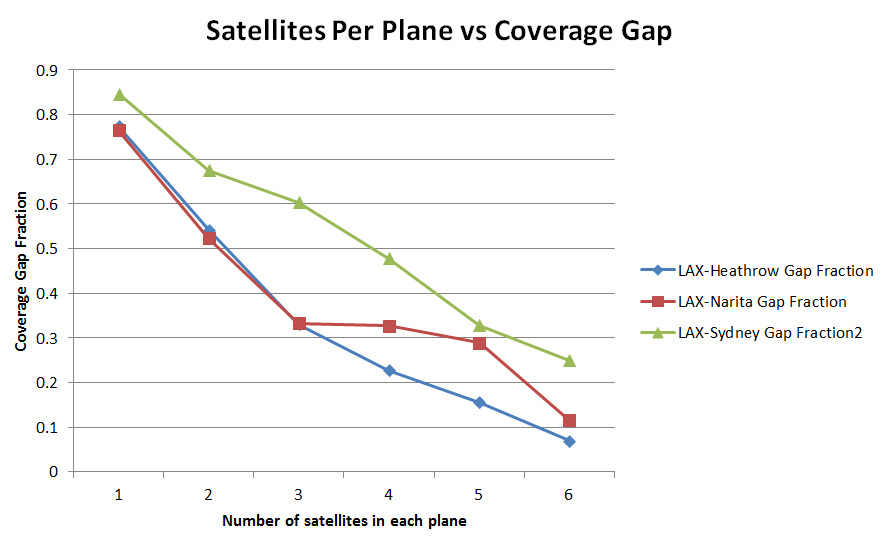
\includegraphics[scale = 0.6]{Pictures/PerPlaneVsCovGap12sat.png}
	
	\caption{Coverage gap (as a fraction of total analysis time) as effected by number of satellites per plane. Lower is better}
	\label{fig:PerPlaneVsCovGap12sat}
\end{figure} 

\begin{figure}[H]
	\centering
	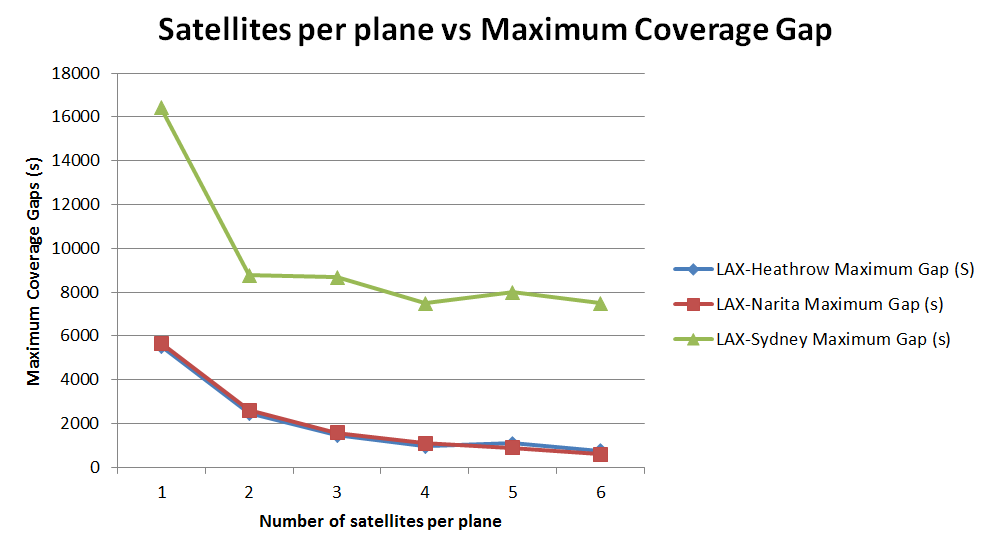
\includegraphics[scale = 0.6]{Pictures/PerPlaneVsMaxGap12sat.png}
	
	\caption{Maximum coverage gap as affected by number of satellites per plane. Lower is better.}
	\label{fig:PerPlaneVsMaxGap12sat}
\end{figure} 

\begin{figure}[H]
	\centering
	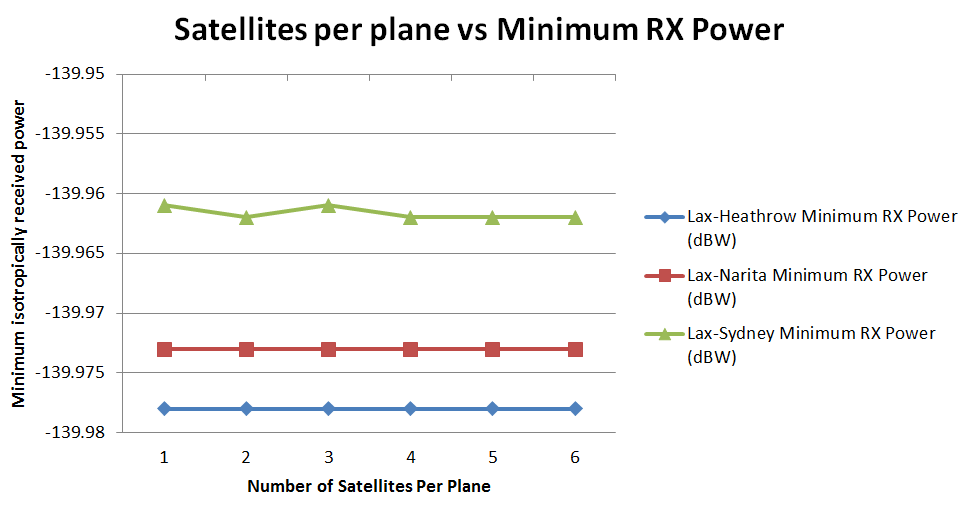
\includegraphics[scale = 0.6]{Pictures/PerPlaneVsRxPower12sat.png}
	
	\caption{Minimum received isotropic power as affected by number of satellites per plane. Higher is better.}
	\label{fig:PerPlaneVsRxPower12sat}
\end{figure}

\subsubsection{Discussion}
As expected, increasing the number of satellites will increase the coverage times available for each flight. Figures \ref{fig:PerPlaneVsCovGap12sat} and \ref{fig:PerPlaneVsMaxGap12sat} show that a higher number of satellites results in less coverage gaps. A higher number of satellites per plane increased the probability with which a given flight was able to see at least one satellite, and also increased the revisit time for a given area on the Earth. The number of satellites in the constellation did not affect the minimum received RF power, as seen in the flatness of Figure \ref{fig:PerPlaneVsRxPower12sat}.

Despite the net beneficial effect on the ADS-B system, the number of satellites needs to be weighed against the cost and maintenance. Increasing the number of satellites did increase the effectiveness of the space based ADS-B coverage constellation. However a higher number of satellites will require an increased launch and maintenance cost, especially when considering the need to distribute the satellites evenly and potential replacement at end of life.


 